

Das Messsignal des VNA setzt sich aus Nutz- und Störsignal zusammen. Letzteres entsteht bspw. durch äußere Einflüsse oder die Temperaturabhängigkeit bestimmter Bauteile. Um eine Abschätzung der Messunsicherheit zu treffen, sollen die Störsignale kurz untersucht werden.
\par
\vspace{\linespace}
Durch eine Messung mit ungeschirmter Messtrecke (vgl. \Abb\ref{subfig:4_Einfuegungsmessung_Fall1}) kann das zufällige Rauschsignal erfasst werden, welches in \Abb\ref{fig:4_Stoersignal} dargestellt ist. Erkennbar ist, dass die Charakteristik tatsächlich der eines zufälligen Rauschsignals entspricht mit einem maximalen Amplitudenbetrag von etwas weniger als \SI{0.075}{\Dezibel} und damit deutlich unter den erwarteten Schirmdämpfungswerten der Proben. Bezogen auf die Feldgrößen entspricht dies nach \Gleichung\eqref{eq:2_Relativer_Pegel_Feldgroessen} einer Messunsicherheit von etwa \SI{0.87}{\percent}. Gegenüber anderen Einflüssen wie sekundären Wellenfronten aufgrund von Reflektionen oder Interferenzen durch Bauteile im Bereich der ersten Fresnelzone ist dies, vor allem im unteren Frequenzbereich, zu vernachlässigen. 
\par


\begin{figure}[ht]
    \centering
    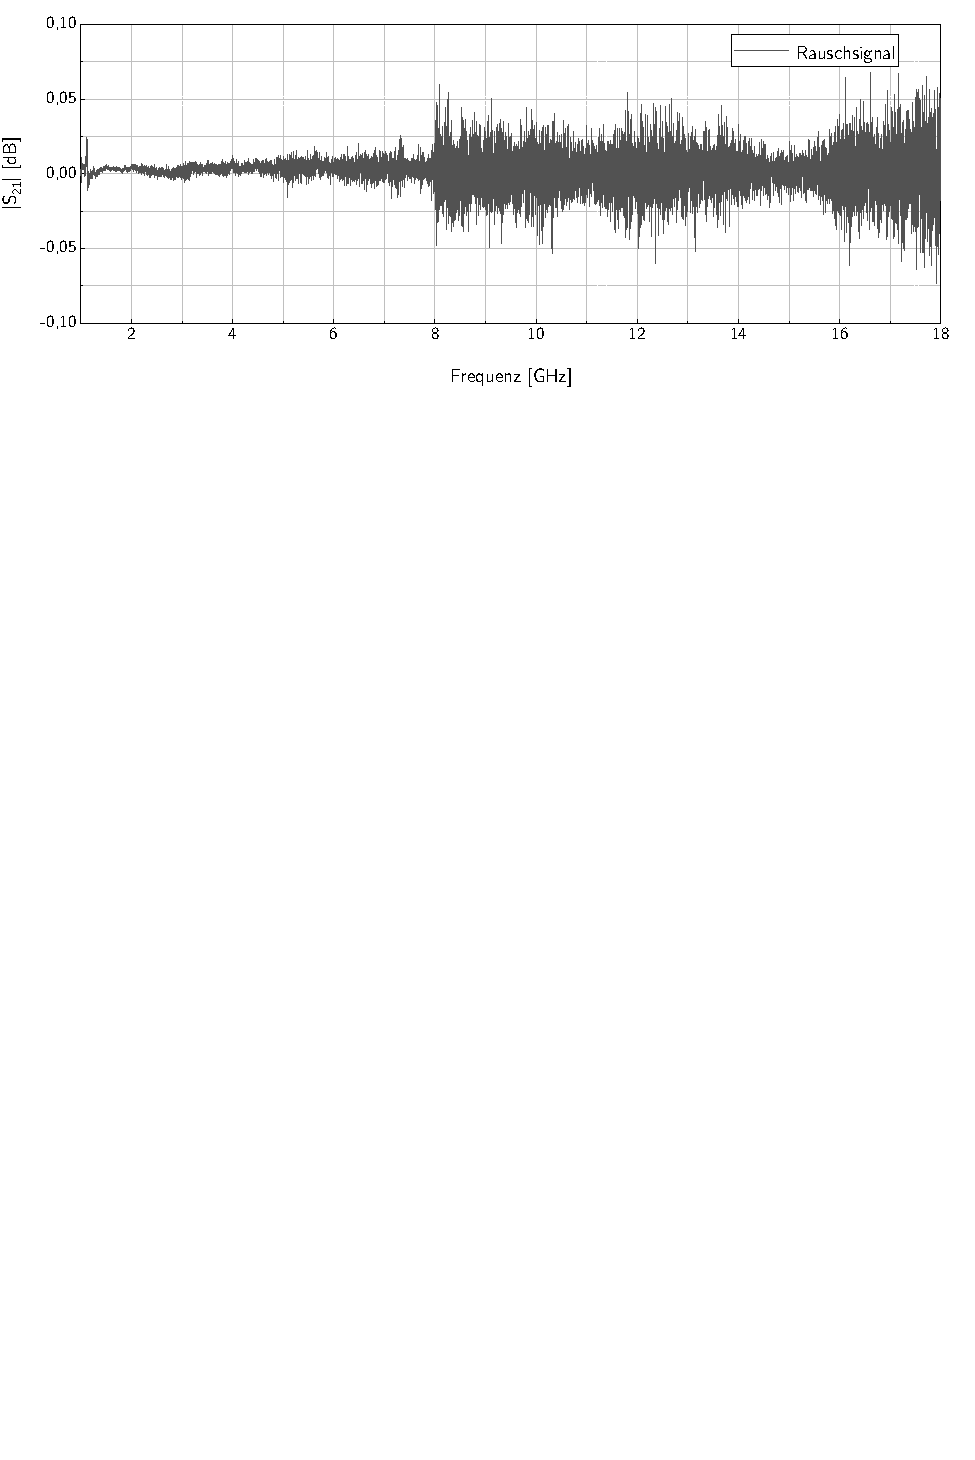
\includegraphics[page = 1, width = .99\textwidth, trim = 0cm 18.05cm 0.3cm 0.05cm, clip]{Abbildungen/Kapitel4/Rauschsignal.pdf}
    \caption{Zufälliges Störsignal des VNA von \SI{1}{\giga\hertz} bis \SI{18}{\giga\hertz}}
    \label{fig:4_Stoersignal}
\end{figure}


Das Rauschsignal weist weiterhin eine deutliche Erhöhung der Amplitude ab ca. \SI{8}{\giga\hertz} auf. Da diese Art von statistischem Rauschen nicht von den Fehlerkorrekturmethoden der Kalibration reduziert wird, könnte dies auf den internen Aufbau des VNA oder auf eine höhere Rauschanfälligkeit der Komponenten zurückzuführen sein. Auf die korrigierbaren Fehlerterme soll im Folgenden kurz eingegangen werden.
% entweder auf den internen Aufbau des VNA oder die verwendete Kalibrationsmethode zurückzuführen sein. Im Folgenden soll deshalb außerdem auf die Kalibration des VNA etwas näher eingegangen werden.
\par
\vspace{\linespace}
In Abhängigkeit von der Anzahl der verwendeten Ports des VNA können unterschiedlich viele Korrekturterme auf die Messung angewandt werden. Hier werden stets beide Ports zur Messung benötigt, sodass nur auf das gängige Korrekturmodell eingegangen werden soll. Da der VNA den Phasor des Messsignals aufzeichnet, können je Port sechs Fehlerterme korrigiert werden~\cite{VNA-Handbuch}. In der \Abb\ref{fig:4_Fehlermodell} ist das vom VNA verwendete Fehlermodell mit den Korrekturtermen $e_{xx}$ für eine vollständige 2-Port Kalibration in Vorwärtsrichtung dargestellt. Wird diese in beide Richtungen angewandt, erhält man die geläufige \mbox{12-Term} Kalibration nach dem aktuellen Stand der Technik~\cite{VNA_Error_Models_and_Calibration_Methods}. Auf die zugrunde liegende Theorie soll an dieser Stelle nicht näher eingegangen werden. Alternativ ist die 1-Pfad-2-Port-Kalibration, welche in der Software des VNA nutzbar ist, ebenfalls ausreichend, wobei bspw. nur die Vorwärts-Koeffizienten der Streumatrix korrigiert werden. 
\par
\vspace{\linespace}


\begin{figure}[ht]
    \centering
    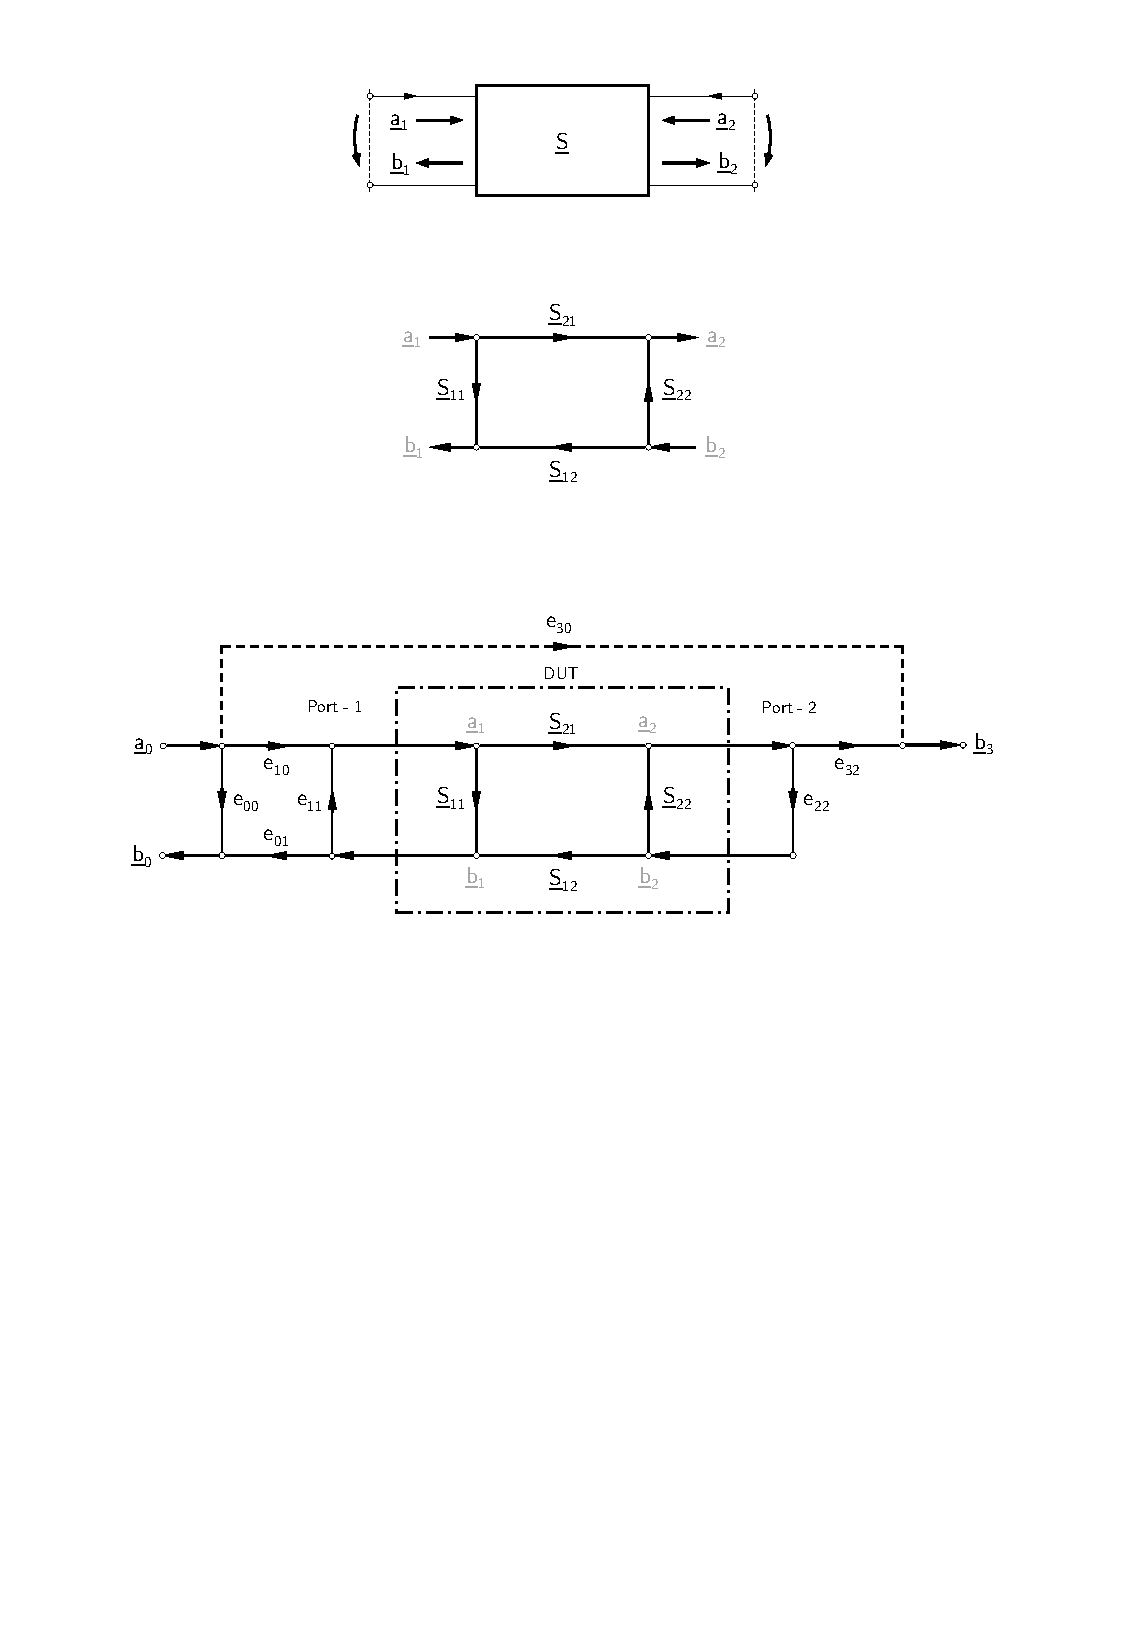
\includegraphics[page = 1, trim = 2cm 12cm 2cm 10.3cm, clip, width = 0.9\textwidth]{Abbildungen/Kapitel4/Zweitor.pdf}
    \caption[Signalflussdiagramm des 12-Term Fehlermodells in Vorwärtsrichtung für zwei Ports]{Signalflussdiagramm des 12-Term Fehlermodells in Vorwärtsrichtung für zwei Ports nach~\cite{VNA_Error_Models_and_Calibration_Methods}}
    \label{fig:4_Fehlermodell}
\end{figure}

Die empfohlene Kalibrationsmethode mithilfe des vorhandenen Kalibration-Kits, das entsprechend hochpräzise definierte Standards enthält, ist die sogenannte SOLT-Kalibration (Short-Open-Load-Through). Dabei werden die Ports des VNA jeweils nacheinander vollständig abgeschlossen, geöffnet und mit einer Last von \SI{50}{\ohm} Wellenwiderstand beaufschlagt. Anschließend werden beide Ports über das Kit miteinander verbunden. Vorteilhaft bei dieser Methode ist, dass sie nicht bandbegrenzt und relativ einfach durchzuführen ist. Die Genauigkeit hängt hier vor allem von der Genauigkeit der definierten Standards ab. Andere Methoden sind jedoch vor allem für sehr hohe Frequenzen etwas genauer~\cite{VNA-Calibration_Application_Note}. 
\par
\vspace{\linespace}
Durchgeführt werden kann die Kalibration natürlich nur an der Schnittstelle der Signalkabel mit den Antennen, sodass die Einflüsse der Antennen nicht korrigiert werden können. Außerdem ist anzumerken, dass zur Durchführung der \glqq Through\grqq-Kalibration nach dieser Methode eine große Lageveränderung der Signalkabel notwendig ist, da diese mithilfe des Kalibrationskits verbunden werden müssen. Dies kann durchaus einen nicht zu vernachlässigenden Einfluss auf das Messsignal haben, sodass ggf. die in~\cite{VNA-Calibration_Application_Note} und~\cite{VNA-Handbuch} beschriebene SOLR-Methode (Short-Open-Load-Reciprocal), welche keine direkte \glqq Through\grqq-Definition benötigt, noch bessere Ergebnisse liefert. Dies wurde im Rahmen dieser Arbeit nicht getestet, könnte aber für fortführende Untersuchungen in Betracht gezogen werden.
\par
\vspace{\linespace}
Zu beachten ist außerdem, dass die Genauigkeit nach erfolgter Kalibration aufgrund von bspw. Drifts abnehmen kann, sodass in Abhängigkeit der Nutzung und Umgebungsbedingungen eine Aktualisierung der gespeicherten Kalibrierung notwendig ist. Da im Labor relativ konstante Umgebungsbedingungen herrschen und die Kalibration nach einer entsprechenden Aufwärmzeit des VNA durchgeführt wurde, verlängert sich die Zeit zwischen den notwendigen Neukalibrierungen~\cite{VNA-Handbuch, VNA_Error_Models_and_Calibration_Methods}. Es wird jedoch empfohlen, diese vor jeder Messkampagne durchzuführen.


%Wie alle Messgeräte --> zufällige SChwankungen
%Charakterisierung des Rauschsignals und kurzer Vergleich mit Größ0enordnung der Messungen


%--> Kalibration zum Ausgleich von Drifts und Offsets gegenüber einem idealen Messgerät

%verschiedene Methoden --> beschreiben

%auf SLOT und Thru eingehen und vergleichen, wann welche Methode sinnvoll ist


%Neukalibration nach Umgebungsbedingungen --> Temperatur und gemetrischen Änderungen; Thru-Update möglich bei erfolgter 2-Port oder 1 Path 2Port Kalibration

%Interpolation beachten bei erfolgter Kalibration --> Wenn aus müssen Messpunkte mit Kalibrationspunkten übereinstimmen, ansonsten wird interpoliert --> aufpassen, dass Signal richtig abgebilet wird!